\documentclass{beamer}
% Load Packages
\usepackage[utf8]{inputenc}
\usepackage{xcolor}
\usepackage{tikz}
\usetikzlibrary{positioning,calc}
\usepackage[absolute,overlay]{textpos}
\usepackage{graphicx}
\usepackage{hyperref}
\usepackage{amsmath}
\usepackage{listings}
\usepackage{fontawesome}
\usepackage[brazilian]{babel}
\usepackage{datetime}
\usepackage{subcaption} % usado para figuras lado a lado

% Define Commands
\newcommand*{\ClipSep}{0.06cm} %To adjust footer logo
\newcommand{\E}{\mathrm{e}\,} %\def\I{e} % used to defined e for exp(x), see later what it should be
\newcommand{\ud}{\mathrm{d}}
\lstset{numbers=left, numberstyle=\tiny, stepnumber=1,firstnumber=1,breaklines=true,
    numbersep=5pt,language=Python,
    stringstyle=\ttfamily,
    basicstyle=\footnotesize, 
    showstringspaces=false
}
 
\usetheme{oxonian}
\setbeamertemplate{itemize subitem}{$-$}
\setbeamertemplate{itemize subsubitem}[circle]
 
\title{Apresentação da Disciplina}
\subtitle{Programação Estruturada e Orientada a Objetos}
\titlegraphic{
\includegraphics[width=2.5cm]{Theme/Logos/ifrn_cm_vertical.png}}
\author{Prof. Me. Leo Moreira Silva}

\date{\today}

\begin{document}

{\setbeamertemplate{footline}{} 
\frame{\titlepage}}

\section*{Agenda}\begin{frame}{Agenda}\tableofcontents\end{frame}

\section{Introdução}

\begin{frame}{Introdução}
    \begin{itemize}
        \item Carga Horária:
        \begin{itemize}
            \item 120 horas
            \item 160 hora/aula
        \end{itemize}
        \item Horário das Aulas:
        \begin{itemize}
            \item 2T12 (1º Semestre)
            \item 3T34 (1º Semestre)
        \end{itemize}
        \item Local:
        \begin{itemize}
            \item Laboratório de Informática I (Sala 216) ou II (Sala 214)
        \end{itemize}
        \item Horário de CA:
        \begin{itemize}
            \item Qualquer dia e horário, a combinar em cada ocasião
        \end{itemize}
    \end{itemize}
\end{frame}


\section{Objetivos}

\begin{frame}{Objetivos}
    \begin{itemize}
        \item Implementar algoritmos
        \item Utilizar vetores, matrizes e registros em programas computacionais
        \item Desenvolver bibliotecas de funções
        \item Implementar aplicações em ambiente gráfico
        \item Aplicar os conceitos básicos de orientação a objetos
        \item Conhecer as coleções de objetos
        \item Desenvolver aplicações usando linguagem de suporte ao Paradigma Orientado a Objetos
        \item Desenvolver aplicações com interfaces gráficas com o usuário e armazenamento persistente
    \end{itemize}
\end{frame}

\section{Conteúdo}

\begin{frame}[allowframebreaks]{Conteúdo}
    \begin{enumerate}
        \item Implementação de algoritmos
        \begin{enumerate}
            \item Conceitos fundamentais
            \item Tipos básicos de dados
            \item Memória, constantes e variáveis
            \item Operadores aritméticos, lógicos e relacionais
            \item Comandos básicos de atribuição, de entrada e saída de dados
            \item Funções primitivas
            \item Estruturas condicionais
            \item Estruturas de repetição
        \end{enumerate}
        \framebreak
        \item Tipos estruturados de dados
        \begin{enumerate}
            \item Strings
            \item Vetores e matrizes
            \item Arquivos de texto
        \end{enumerate}
        \item Modularidade
        \begin{enumerate}
            \item Métodos estáticos (funções)
            \item Passagem de parâmetros (por valor e referência)
            \item Bibliotecas de vínculo estático
        \end{enumerate}
        \framebreak
        \item Introdução à orientação a objetos
        \begin{enumerate}
            \item Objetos, classes, referências, diagramas de classes
            \item Estado, comportamento, identidade, abstração e encapsulamento
            \item Atributos, métodos e construtores
            \item Herança e polimorfismo
            \item Interfaces
        \end{enumerate}
        \item Tratamento de Exceções
        \item Pacotes e espaços de nomes
        \framebreak
        \item Coleções de objetos
        \begin{enumerate}
            \item Listas, conjuntos e mapas
            \item Tipos genéricos
        \end{enumerate}
        \item Serialização e persistência de objetos
        \begin{enumerate}
            \item Serialização de objetos
            \item Arquivos e fluxos
        \end{enumerate}
        \item Interfaces gráficas com o usuário
    \end{enumerate}
\end{frame}

\section{Procedimentos Metodológicos}

\begin{frame}{Procedimentos Metodológicos}
    \begin{itemize}
        \item Aulas teóricas expositivas
        \item Aulas práticas em laboratório
        \item Desenvolvimento de projetos
    \end{itemize}
\end{frame}

\begin{frame}{Procedimentos Metodológicos}
    \begin{itemize}
        \item Técnica \textbf{Pomodoro}
        \begin{itemize}
            \item Melhora a agilidade do cérebro, estimular o foco, maximizar a aprendizagem e a concentração
            \item 15 minutos de \textbf{foco máximo}
            \begin{itemize}
                \item Sem \textbf{interrupções} de nenhuma ordem (celular, computador, redes sociais, banheiro, etc)
            \end{itemize}
            \item 5 minutos de \textbf{descanso}
        \end{itemize}
    \end{itemize}
    \begin{figure}
        
\includegraphics[width=2.5cm]{Theme/Logos/pomodoro-technique.png}
    \end{figure}
\end{frame}

\section{Avaliações}

\begin{frame}{Avaliações}
    \begin{itemize}
        \item Avaliações escritas
        \item Avaliações práticas
        \item Trabalhos
    \end{itemize}
\end{frame}

\section{Software de Apoio}

\begin{frame}[allowframebreaks]{Software de Apoio}
    \begin{itemize}
        \item Edmodo
        \begin{itemize}
            \item Rede social educacional
            \item Permite a comunicação entre professores e alunos
            \item Ideal para comunicação e colaboração
            \item Irmão educativo do Facebook
            \item Professor pode submeter trabalhos, enquetes
            \item Armazenamento de arquivos
        \end{itemize}
    \end{itemize}
    \begin{figure}
        
\includegraphics[width=1.5cm]{Theme/Logos/edmodo_logo.png}
    \end{figure}
    \framebreak
    \begin{itemize}
        \item https://www.edmodo.com
    \end{itemize}
    \begin{figure}
        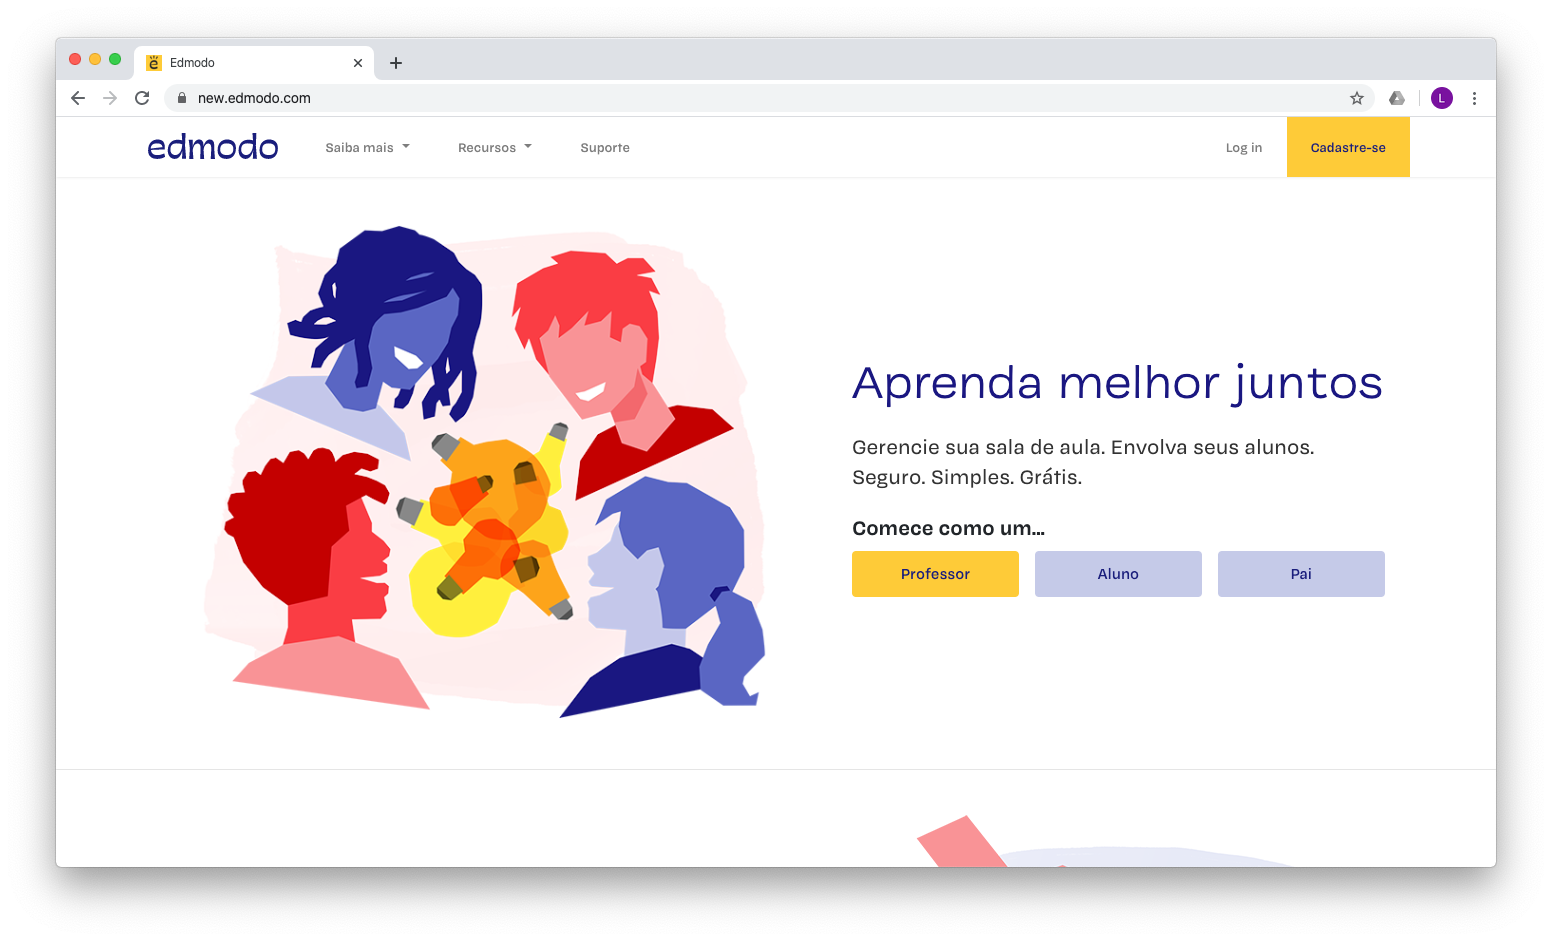
\includegraphics[scale=0.17]{Theme/Logos/tela_inicial_edmodo.png}
    \end{figure}
    \framebreak

    \begin{columns}
        \column{0.5\textwidth}
            \begin{itemize}
                \item Código da classe: \textbf{2r4cin}
            \end{itemize}
        \column{0.5\textwidth}
            \begin{figure}
                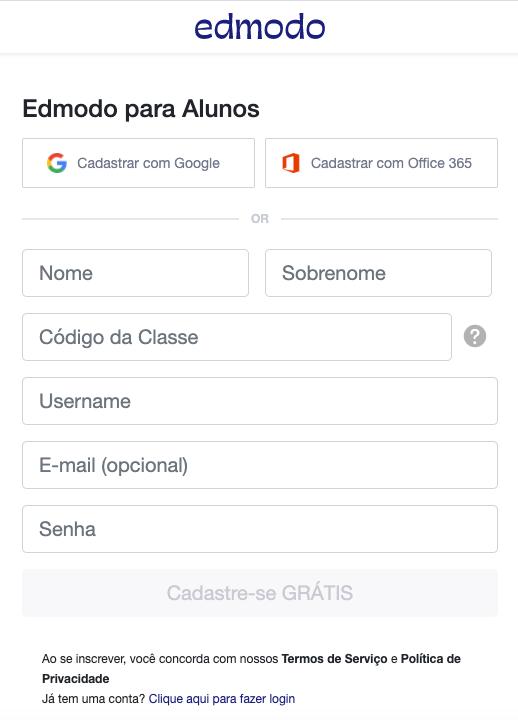
\includegraphics[scale=0.26]{Theme/Logos/edmodo_inicio_aluno.png}
            \end{figure}
    \end{columns}
    \framebreak

    \begin{columns}
        \column{0.5\textwidth}
            \begin{itemize}
                \item PyCharm
            \end{itemize}
        \column{0.5\textwidth}
            \begin{figure}
                
\includegraphics[scale=0.07]{Theme/Logos/pycharm_logo.png}
            \end{figure}
    \end{columns}

\end{frame}

\section{Bibliografia}

\begin{frame}{Bibliografia}
    \begin{enumerate}
        \item MIZRAHI, Victorine V. Treinamento em linguagem C - Módulo 1. Prentice Hall, 2005.
        \item MIZRAHI, Victorine V. Treinamento em linguagem C - Módulo 2. Prentice Hall, 2004.
        \item DEITEL, H. M.; DEITEL, P. J. Java: como programar. 4a Edição. Bookman, 2003.
        \item SHARP, John. Microsoft Visual C\# 2008: Passo a passo. Bookman, 2008.
        \item \textbf{Materiais disponibilizados pelo professor}
    \end{enumerate}
\end{frame}

\section{Livros na Biblioteca}

\begin{frame}[allowframebreaks]{Livros na Biblioteca}
    \begin{figure}[H]
        \centering
         \begin{subfigure}{.5\textwidth}
            \centering
            \frame{
\includegraphics[scale=0.3]{Theme/Logos/python_cookbook.jpg}}
            \textsf{\caption{Python Cookbook}}
         \end{subfigure}%
         \begin{subfigure}{.5\textwidth}
            \centering
            \frame{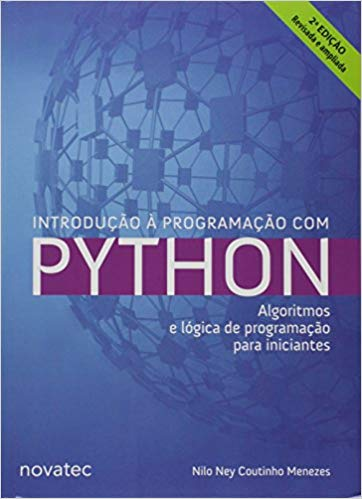
\includegraphics[scale=0.24]{Theme/Logos/introducao_programacao_python.jpg}}
            \textsf{\caption{Introdução à Programação com Python}}
         \end{subfigure}
    \end{figure}
    \framebreak
    \begin{figure}
        \frame{
\includegraphics[scale=0.24]{Theme/Logos/python_sbc.jpg}}
            \textsf{\caption{Introdução à Algoritmos e Programação com Python}}
    \end{figure}
\end{frame}

\section{Regras}

\begin{frame}{Regras}
    \begin{itemize}
        \item Principal e fundamental: \textbf{diálogo}
        \item Outras regras:
        \begin{itemize}
            \item Ser assíduo e pontual
            \item Desligar o celular ou mante-lo no modo silencioso
            \item Participar ativamente, estudar em casa e tirar dúvidas
            \item Respeitar os colegas
            \item Datas de entregas de atividades não serão estendidas (exceto por vontade do professor)
            \item Entregas atrasadas não serão permitidas
            \item Ser ético, sincero e honesto
            \item \dots
        \end{itemize}
    \end{itemize}
\end{frame}

\begin{frame}{Qual o segredo da disciplina?}
    \begin{figure}
        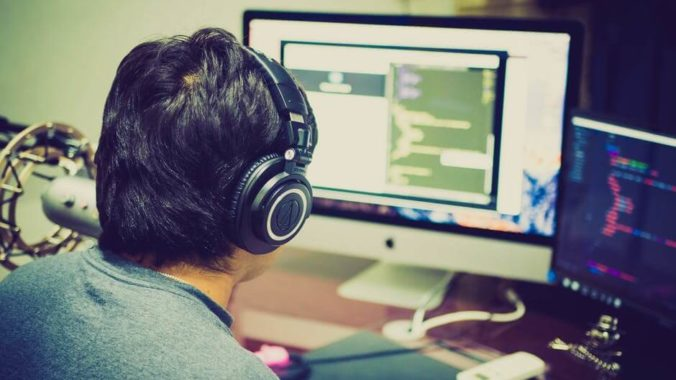
\includegraphics[scale=0.4]{Theme/Logos/praticar.jpeg}
    \end{figure}
\end{frame}

\begin{frame}{Dúvidas?}
    \begin{figure}
        
\includegraphics[scale=0.35]{Theme/Logos/duvidas_frequentes.png}
    \end{figure}
\end{frame}

\end{document}